\documentclass[12pt,a4paper,oneside]{report}

\usepackage[top=3cm,bottom=3cm,left=4cm,right=3cm]{geometry}
\usepackage{times}
% tanpa babel (pola hyphenation default sudah cukup)
\usepackage{graphicx}
\usepackage{tabularx}
\usepackage{booktabs}
\usepackage{enumitem}
\usepackage{amsmath}
\usepackage{fancyhdr}
\usepackage{titlesec}
\usepackage{setspace}
\usepackage[hidelinks,pdfencoding=unicode]{hyperref}

\onehalfspacing
\pagestyle{fancy}
\fancyhf{}
\fancyhead[R]{\small\textit{Proposal Seminar Nasional --- ANDROMEDA}}
\fancyfoot[C]{\thepage}
\renewcommand{\headrulewidth}{0.4pt}

\titleformat{\chapter}[hang]{\Large\bfseries}{BAB \thechapter\enspace}{0pt}{}
\titlespacing*{\chapter}{0pt}{0pt}{18pt}

\hyphenation{ir-i-ga-si mo-ni-to-ring kon-fi-gu-ra-si thres-hold sen-sor esp32}

\begin{document}

% ================= COVER =================
\begin{titlepage}
\centering
\vspace*{1.5cm}
{\large\textbf{PROPOSAL SEMINAR NASIONAL}}\\[0.4cm]
{\small\textit{Rancang Bangun Sistem Cerdas Berbasis Internet of Things}}\\[1.2cm]
{\Large\bfseries Rancang Bangun Irigasi Tetes Multi-Zona Berbasis ESP32 dengan Kendali Dual-Threshold dan Monitoring Android}\\[0.6cm]
{\large ANDROMEDA: \textit{Android Routine Monitoring Electronic Drip Automation}}\\[1.5cm]
\begin{tabular}{ll}
Penulis & : \textbf{FARREL GHOZY AFIFUDIN (452024611053)} \\
Anggota 1 & : M. FARIDH MAULANA (452024611065) \\
Anggota 2 & : MUSTAQIM NAWAHHUDI MA'ARIF (452024611037) \\
Program Studi & : Teknik Informatika \\
Institusi & : Universitas Darussalam Gontor \\
Lokus Penelitian & : Desa Merayan (Program Desa Binaan) \\
\end{tabular}\\[1.5cm]
{\small Disusun sebagai proposal makalah Seminar Nasional (luar kampus)\\Oktober 2026}\\[2cm]
\vfill
{\small Sistem: 1 ESP32 mengelola 6 zona $\cdot$ Dual-threshold 30\%/70\% $\cdot$ Supabase $\cdot$ Flutter Android offline-first $\cdot$ Open-Meteo}
\end{titlepage}

\pagenumbering{roman}
\tableofcontents
\clearpage
\pagenumbering{arabic}

% ================= ABSTRAK =================
\chapter*{Abstrak}
\addcontentsline{toc}{chapter}{Abstrak}

Irigasi manual pada lahan kering pedesaan boros air dan menuntut kehadiran petani setiap hari, sementara konektivitas internet desa yang intermiten membuat banyak sistem \textit{smart farming} berbasis cloud gagal beroperasi stabil. Penelitian ini merancang-bangun \textbf{ANDROMEDA} (\textit{Android Routine Monitoring Electronic Drip Automation}), sistem irigasi tetes otomatis multi-zona untuk 6 petak yang dikelola oleh \textbf{satu node ESP32}: enam sensor kelembaban tanah kapasitif (GPIO 32, 33, 34, 35, 36, 39) dan enam relay solenoid valve (GPIO 26, 27, 14, 12, 13, 15), dengan backend Supabase (PostgreSQL + REST + Realtime) dan aplikasi Android Flutter yang \textit{offline-first} serta terintegrasi prakiraan cuaca Open-Meteo. Kontribusi utama penelitian ini adalah: (1) arsitektur \textit{single-node multi-zone} berbiaya rendah, (2) kendali histeresis \textit{dual-threshold} (kering 30\%, basah 70\%) untuk mencegah valve berosilasi, dan (3) mekanisme \textit{heartbeat} 60 detik plus \textit{cache snapshot} lokal untuk ketahanan konektivitas intermiten. Evaluasi dirancang atas enam aspek: fungsionalitas valve, akurasi logika threshold, latensi perintah HP ke solenoid, akurasi status online/offline, efisiensi penggunaan air dibanding penyiraman manual, dan keberterimaan petani (SUS). Luaran yang ditargetkan adalah makalah seminar nasional, prototipe teruji di Desa Merayan, aplikasi Android, dan dataset pembacaan sensor.

\textbf{Kata kunci:} irigasi tetes, multi-zona, ESP32, dual-threshold, histeresis, Supabase, Android offline-first, heartbeat, Open-Meteo.

\vspace{0.6cm}
\begin{center}\textbf{\textit{Abstract}}\end{center}
\textit{Manual irrigation in rural drylands wastes water and demands daily farmer presence, while intermittent village connectivity destabilizes many cloud-based smart farming systems. This study designs and implements ANDROMEDA (Android Routine Monitoring Electronic Drip Automation), an automatic multi-zone drip irrigation system in which a single ESP32 node manages six beds: six capacitive soil-moisture sensors and six solenoid-valve relays, backed by Supabase (PostgreSQL + REST + Realtime) and an offline-first Flutter Android app integrated with the Open-Meteo weather forecast. The main contributions are: (1) a low-cost single-node multi-zone architecture, (2) dual-threshold hysteresis control (dry 30\%, wet 70\%) preventing valve chattering, and (3) a 60-second heartbeat plus local cache snapshot for resilience under intermittent connectivity. Evaluation covers valve functionality, threshold-logic accuracy, phone-to-solenoid command latency, online/offline status accuracy, water-use efficiency versus manual watering, and farmer acceptance (SUS). Expected outputs are a national-seminar paper, a field-tested prototype in Merayan Village, the Android app, and a sensor-reading dataset.}

\textit{\textbf{Keywords:} drip irrigation, multi-zone, ESP32, dual-threshold, hysteresis, Supabase, offline-first Android, heartbeat, Open-Meteo.}

% ================= BAB 1 =================
\chapter{Pendahuluan}

\section{Latar Belakang}
Air adalah faktor pembatas utama produktivitas lahan kering. Irigasi tetes (\textit{drip irrigation}) dikategorikan FAO sebagai teknologi \textit{climate-smart agriculture} karena menghantarkan air dan nutrisi secara presisi ke zona perakaran sehingga jauh lebih hemat dibanding penyiraman permukaan/manual \cite{fao-drip}. Namun adopsi di tingkat petani desa terhambat tiga hal: biaya perangkat, kebutuhan listrik dan internet yang stabil, serta pengoperasian yang rumit.

Perkembangan mikrokontroler murah ber-WiFi seperti ESP32 membuka peluang otomatisasi berbiaya rendah \cite{espressif-datasheet}. Sensor kelembaban tanah kapasitif versi murah (v1.2) banyak dipakai, tetapi memerlukan kalibrasi yang benar agar konsisten untuk manajemen irigasi; Abdelmoneim dkk. menunjukkan bahwa sensor kapasitif berbiaya rendah harus dikalibrasi dan diuji konsistensinya sebelum diintegrasikan ke sistem monitoring IoT \cite{abdelmoneim2025}. Di sisi sistem, Saputri dkk. merancang-bangun monitoring dan kendali irigasi berbasis Blynk IoT dan ThingSpeak \cite{saputri2025}, sedangkan Fahrunnisa dkk. membangun sistem irigasi inovatif untuk cabai memakai bot Telegram dan dasbor web \cite{fahrunnisa2026}. Kedua sistem tersebut valid, tetapi bertumpu pada pola umum: satu node per titik, kendali on/off ambang tunggal, dan ketergantungan penuh pada koneksi cloud.

ANDROMEDA yang dikembangkan penulis mengambil jalur berbeda untuk konteks Desa Merayan (Program Desa Binaan): \textbf{satu ESP32 mengelola enam petak sekaligus}, kendali \textbf{dual-threshold} 30\%/70\% berprinsip histeresis agar valve tidak hidup-mati berulang di sekitar satu titik ambang, \textbf{heartbeat tiap 60 detik} untuk status online/offline yang akurat, backend Supabase sebagai \textit{single source of truth} (4 tabel: \textit{devices}, \textit{sensor\_readings}, \textit{pending\_commands}, \textit{system\_config}), dan aplikasi Android Flutter yang \textbf{offline-first} (snapshot cache lokal + banner offline) serta terintegrasi prakiraan cuaca Open-Meteo yang gratis tanpa \textit{API key} \cite{openmeteo-docs} dan beroperasi di atas dokumentasi Supabase yang terbuka \cite{supabase-docs}. Tenaga berasal dari aki 100Ah + panel surya 300Wp sehingga \textit{off-grid}, dan internet memakai router 4G LTE seharga Rp15.000/bulan. Prototipe perangkat lunak telah mencapai versi aplikasi v0.2.0 (cuaca, jurnal petani, rekapan data, offline mode); yang diajukan pada seminar ini adalah rancang-bangun lengkap beserta evaluasi terukurnya.

\section{Rumusan Masalah}
Berdasarkan latar belakang tersebut, rumusan masalah penelitian ini adalah:
\begin{enumerate}[leftmargin=1.2cm]
\item Bagaimana merancang arsitektur \textit{single-node} ESP32 yang stabil untuk membaca 6 sensor dan mengendalikan 6 solenoid valve secara independen?
\item Apakah kendali histeresis dual-threshold (kering 30\%, basah 70\%) mencegah osilasi valve dan menjaga kelembaban tiap zona pada rentang yang diinginkan?
\item Bagaimana mekanisme heartbeat dan cache snapshot menjamin status perangkat yang akurat serta aplikasi tetap berguna saat internet desa terputus?
\item Berapa efisiensi penggunaan air dan latensi perintah sistem dibanding penyiraman manual, serta bagaimana keberterimaan petani?
\end{enumerate}

\section{Tujuan Penelitian}
\begin{enumerate}[leftmargin=1.2cm]
\item Membangun sistem irigasi tetes 6 zona berbasis satu ESP32, backend Supabase, dan aplikasi Android monitoring-kendali.
\item Mengimplementasikan dan menguji kendali dual-threshold 30\%/70\% yang dapat dikonfigurasi per zona dari aplikasi.
\item Mengimplementasikan heartbeat 60 detik dan mode offline-first (snapshot cache, banner offline, penonaktifan tombol valve saat luring).
\item Mengukur efisiensi air, latensi perintah, akurasi status online/offline, dan skor keberterimaan petani (SUS).
\end{enumerate}

\section{Manfaat Penelitian}
\textbf{Teoretis:} memberikan bukti empiris bahwa arsitektur single-node multi-zone dengan histeresis dan heartbeat layak untuk irigasi IoT murah di daerah konektivitas intermiten. \textbf{Praktis:} petani Desa Merayan menghemat air dan kunjungan lahan; biaya replikasi rendah (elektronik inti $\pm$Rp710 ribu per unit pengendali di luar daya dan router). \textbf{Institusional:} mendukung Program Desa Binaan UNIDA Gontor dengan teknologi tepat guna yang sumber kodenya terbuka (MIT).

\section{Batasan Masalah}
\begin{enumerate}[leftmargin=1.2cm]
\item Lokus: 1 lahan, 6 petak (Lahan A, Desa Merayan); 1 ESP32 (esp32-01).
\item Sensor: capacitive soil v1.2, kalibrasi dua titik (ADC 2700 = kering 0\%, 1500 = basah 100\%; rentang valid 100--4000, di luar itu dinyatakan SENSOR ERROR).
\item Aktuator: solenoid valve 12V NC via relay 1 kanal; sumber air tandon gravitasi (tanpa pompa).
\item Daya: aki 100Ah + surya 300Wp; internet router 4G LTE.
\item Aplikasi: Android (Flutter); cuaca memakai Open-Meteo; jurnal dan cache tersimpan lokal.
\end{enumerate}

\section{Kontribusi / Novelty}
Dibanding penelitian terkait \cite{saputri2025,fahrunnisa2026}, novelty yang diklaim dan akan diuji adalah gabungan empat hal dalam satu sistem: (1) single-ESP32 untuk 6 zona independen; (2) dual-threshold terkonfigurasi per zona; (3) heartbeat + \textit{last\_seen} sebagai penentu status online yang terukur; (4) offline-first + rekomendasi irigasi berbasis prakiraan hujan pada aplikasi petani.

% ================= BAB 2 =================
\chapter{Kajian Pustaka}

\section{Irigasi Tetes}
Irigasi tetes mengalirkan air bertekanan rendah melalui emitter ke zona perakaran. FAO menempatkannya dalam katalog teknologi pertanian cerdas iklim karena presisi pemberian air dan nutrisi (fertigasi) \cite{fao-drip}. Hipotesis yang diuji dalam penelitian ini: otomatisasi berbasis kelembaban memangkas volume air dibanding penyiraman manual terjadwal.

\section{Mikrokontroler ESP32}
ESP32 adalah mikrokontroler 32-bit ber-WiFi/Bluetooth dengan ADC 12-bit multi-kanal, cocok untuk membaca banyak sensor analog \cite{espressif-datasheet}. ANDROMEDA memakai seluruh ADC1 (GPIO 32, 33, 34, 35, 36, 39) untuk 6 sensor dan pin digital (26, 27, 14, 12, 13, 15) untuk 6 relay. Pemilihan ADC1 disengaja karena ADC2 terganggu saat WiFi aktif.

\section{Sensor Kelembaban Kapasitif v1.2 dan Kalibrasi}
Sensor kapasitif mengukur konstanta dielektrik tanah sehingga tidak mudah korosi seperti sensor resistif YL-69. Namun pembacaan mentah (ADC) tidak linear antar unit tanah, sehingga kalibrasi wajib \cite{abdelmoneim2025}. Penelitian ini memakai kalibrasi dua titik dari firmware: nilai ADC 2700 dipetakan ke 0\% (kering) dan 1500 ke 100\% (basah), dengan validasi rentang 100--4000; di luar rentang dianggap kabel putus/sensor error dan tidak di-plot pada grafik.

\section{Kendali Dual-Threshold (Histeresis)}
Kendali ambang tunggal menyebabkan \textit{chattering}: valve hidup-mati cepat saat kelembaban berfluktuasi di sekitar ambang. Dual-threshold memberi celah histeresis: siram mulai saat kelembaban $< 30$\% (threshold\_dry), berhenti saat $> 70$\% (threshold\_wet), diam di antaranya. Nilai default 30/70 tersimpan per zona pada tabel \textit{system\_config} dan dapat diubah petani dari aplikasi sesuai tanaman.

\begin{figure}[h]
\centering
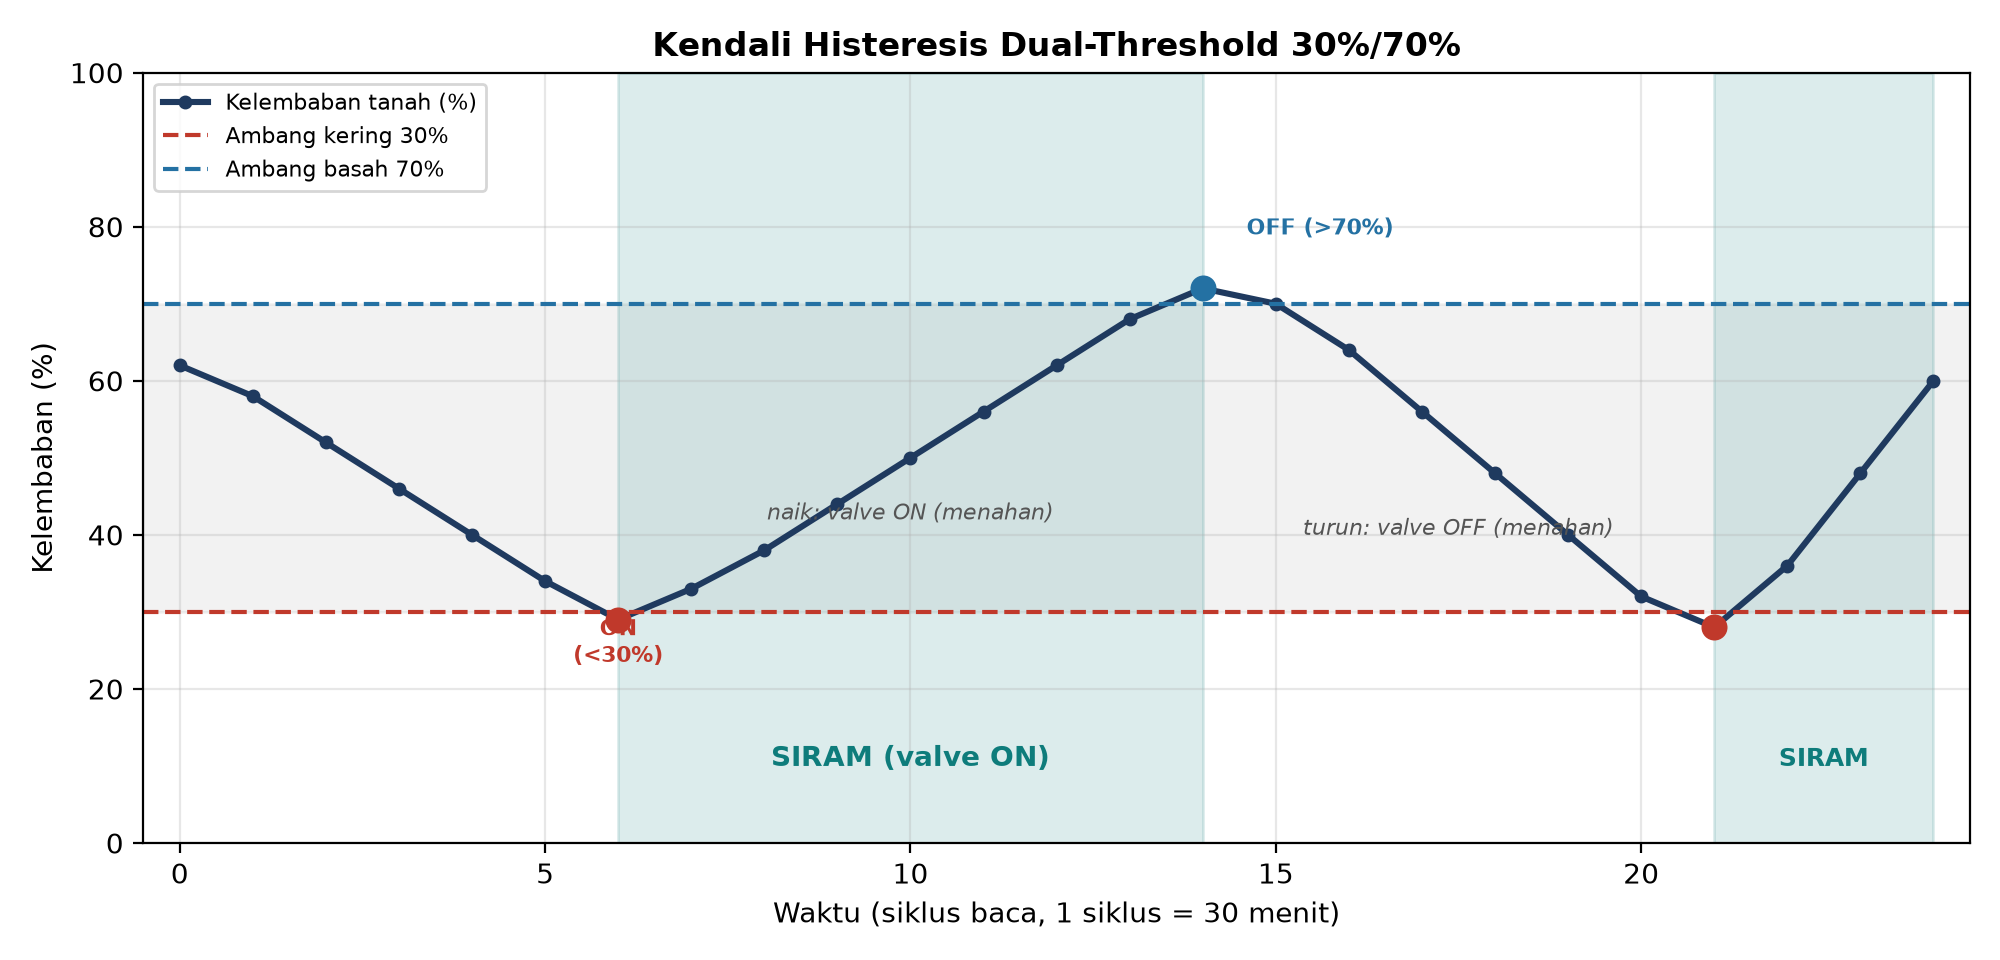
\includegraphics[width=\textwidth]{figures/fig4_threshold.png}
\caption{Ilustrasi kendali histeresis dual-threshold 30\%/70\%: valve ON saat kelembaban jatuh di bawah 30\% dan ditahan ON selama naik sampai menembus 70\%, lalu OFF dan ditahan selama turun (mencegah \textit{chattering}).}
\label{fig:histeresis}
\end{figure}

\section{Backend Supabase}
Supabase menyediakan PostgreSQL, REST API otomatis, dan Realtime WebSocket \cite{supabase-docs}. Skema ANDROMEDA terdiri dari: \textit{devices} (6 petak + \textit{last\_seen}), \textit{sensor\_readings} (log kelembaban + status valve), \textit{pending\_commands} (antrean VALVE\_ON/OFF berstatus pending/executed/expired/cancelled), dan \textit{system\_config} (mode auto/manual, threshold, durasi valve, interval baca). Trigger \textit{touch\_device\_last\_seen} memperbarui \textit{last\_seen} setiap ada bacaan baru sebagai cadangan heartbeat.

\section{Aplikasi Android Offline-First dan Cuaca Open-Meteo}
Aplikasi Flutter menyediakan dasbor real-time, kontrol valve manual, pengaturan threshold, grafik historis, rekapan semua sensor, jurnal dan pustaka pengetahuan petani (100\% lokal), serta prakiraan 7 hari + rekomendasi irigasi dari Open-Meteo. Open-Meteo dipilih karena gratis, tanpa API key/registrasi, dan berlisensi data terbuka CC BY 4.0 \cite{openmeteo-docs}. Prinsip offline-first: setiap refresh sukses menulis snapshot (devices + readings + timestamp) ke SharedPreferences; saat luring, aplikasi tetap terbuka menampilkan data tersimpan + banner, dan tombol valve dinonaktifkan dengan pesan yang jelas.

\section{Heartbeat dan Status Online}
ESP32 mengirim heartbeat tiap 60 detik yang memperbarui \textit{last\_seen}; aplikasi menilai online/offline dari selisih waktu tersebut, bukan dari ada-tidaknya data terakhir. Ini membuat status dapat diuji akurasinya secara kuantitatif (dibanding \textit{ground truth} catu daya ESP32 on/off).

\section{Penelitian Terkait dan Posisi Penelitian Ini}
\begin{table}[h]
\centering
\caption{Perbandingan penelitian terkait.}
\begin{tabularx}{\textwidth}{lXXX}
\toprule
Aspek & Saputri dkk. \cite{saputri2025} & Fahrunnisa dkk. \cite{fahrunnisa2026} & Usulan (ANDROMEDA) \\
\midrule
Node per zona & Umumnya 1 node per titik & 1 node per area & \textbf{1 ESP32 untuk 6 zona} \\
Kendali & Monitoring + kontrol via Blynk/ThingSpeak & Telegram bot + dasbor web & \textbf{Dual-threshold per zona + mode auto/manual} \\
Status online & Tidak dibahas khusus & Tidak dibahas khusus & \textbf{Heartbeat 60 dtk + last\_seen terukur} \\
Ketahanan luring & Tergantung cloud & Tergantung cloud & \textbf{Offline-first + snapshot cache} \\
Konteks & Uji prototipe & Budidaya cabai & \textbf{Off-grid surya, 6 petak Desa Merayan} \\
\bottomrule
\end{tabularx}
\end{table}

% ================= BAB 3 =================
\chapter{Metode Penelitian}

\section{Lokasi dan Objek}
Penelitian dilaksanakan di lahan 1 $\times$ 6 petak (Lahan A) Desa Merayan. Objek: 1 unit ESP32-01, 6 sensor kapasitif, 6 relay + solenoid 12V NC, tandon gravitasi, aki 100Ah + surya 300Wp + SCC 20A, router 4G LTE, backend Supabase, dan aplikasi Android v0.2.0.

\section{Arsitektur Sistem}
Empat lapis: (1) \textbf{Daya}: surya 300Wp $\rightarrow$ SCC 20A $\rightarrow$ aki 100Ah $\rightarrow$ step-down 5V (ESP32 + relay) dan 12V langsung (valve + router). (2) \textbf{Edge}: ESP32 membaca sensor tiap 30 menit (default, konfigurasibel), POST ke Supabase, GET konfigurasi dan antrean perintah, mengeksekusi valve, heartbeat 60 detik. (3) \textbf{Cloud}: Supabase sebagai antrian perintah dan kebenaran tunggal. (4) \textbf{Mobile}: Flutter membaca Realtime, mengirim perintah VALVE\_ON/OFF, mengatur mode dan threshold.

\begin{figure}[h]
\centering
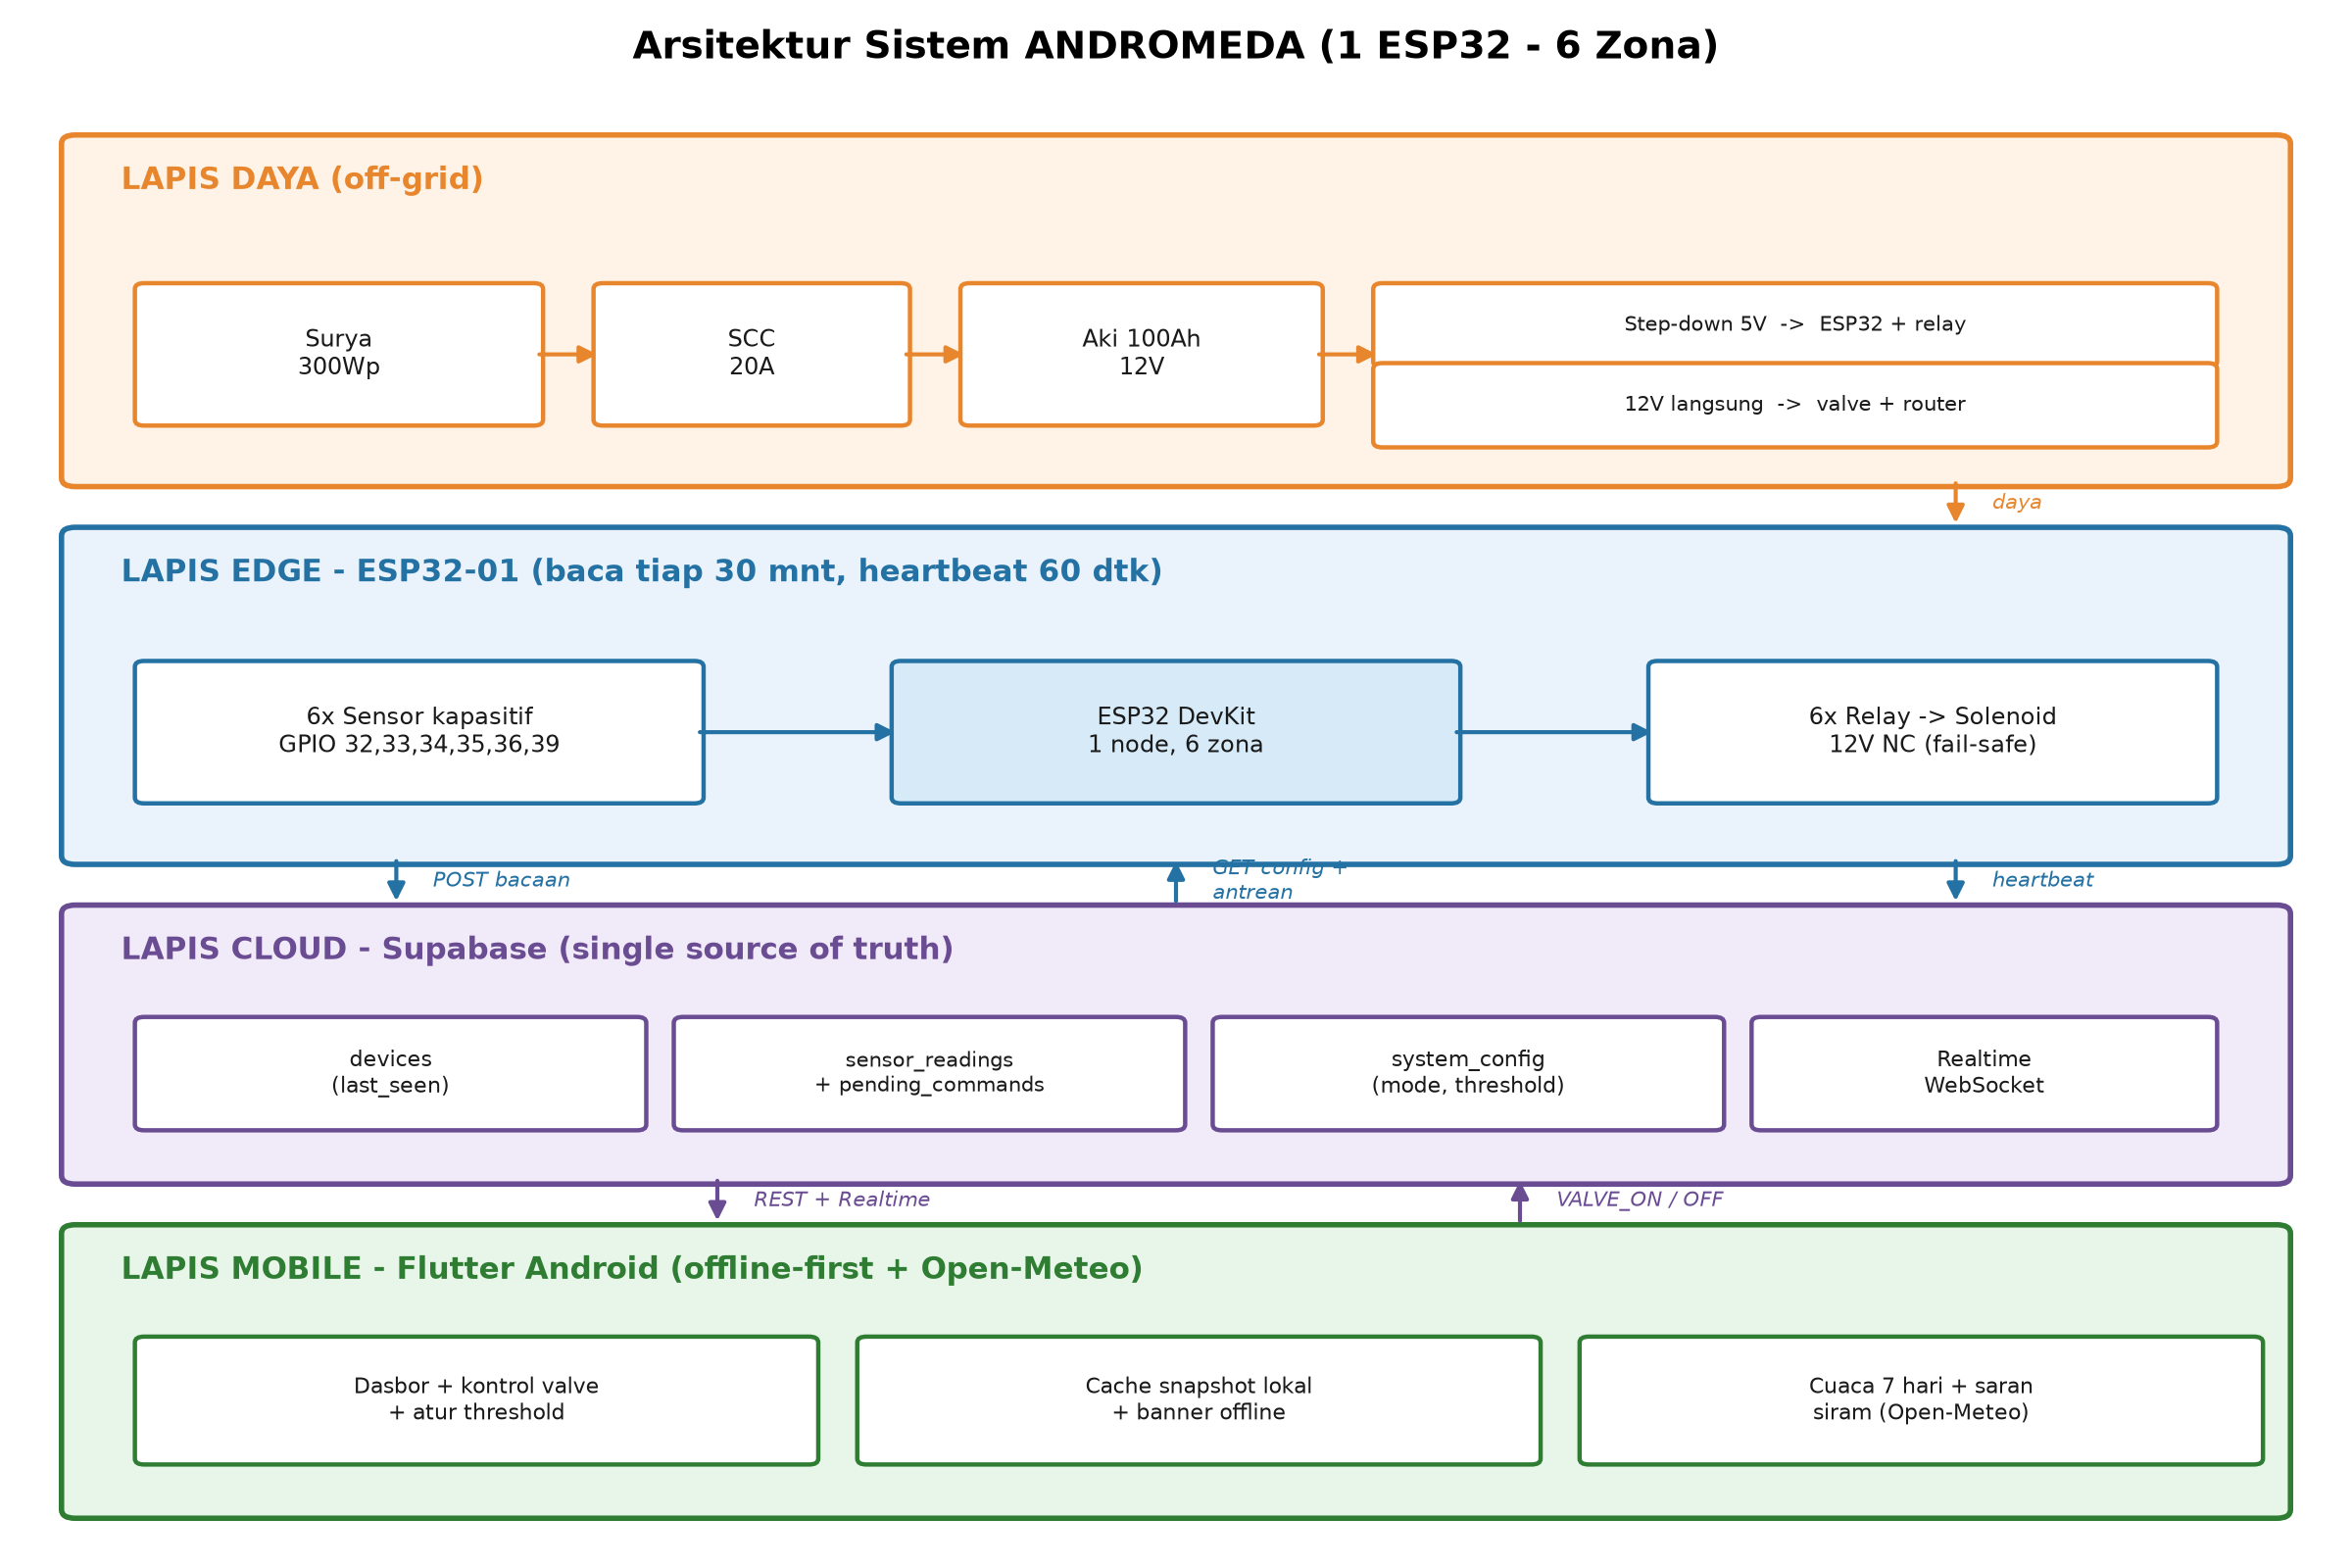
\includegraphics[width=\textwidth]{figures/fig1_arsitektur.png}
\caption{Arsitektur sistem ANDROMEDA empat lapis: daya off-grid, edge single-ESP32, cloud Supabase, dan mobile Android offline-first. Perintah aplikasi antre di \textit{pending\_commands} lalu dieksekusi ESP32.}
\label{fig:arsitektur}
\end{figure}

\section{Perangkat Keras}
\begin{table}[h]
\centering
\caption{Pin ESP32-01 final (1 lahan, 6 petak).}
\begin{tabular}{llll}
\toprule
Petak & Sensor (ADC1) & Relay (digital) & Fungsi \\
\midrule
petak-01 & GPIO 32 & GPIO 26 & Sensor 1 + Valve 1 \\
petak-02 & GPIO 33 & GPIO 27 & Sensor 2 + Valve 2 \\
petak-03 & GPIO 34 & GPIO 14 & Sensor 3 + Valve 3 \\
petak-04 & GPIO 35 & GPIO 12 & Sensor 4 + Valve 4 \\
petak-05 & GPIO 36 & GPIO 13 & Sensor 5 + Valve 5 \\
petak-06 & GPIO 39 & GPIO 15 & Sensor 6 + Valve 6 \\
\midrule
\multicolumn{4}{l}{LED indikator: GPIO 2 (built-in). Sensor: OUT$\rightarrow$GPIO, VCC$\rightarrow$3.3V, GND$\rightarrow$GND.} \\
\multicolumn{4}{l}{Relay: IN$\rightarrow$GPIO (HIGH=ON), VCC$\rightarrow$5V, COM$\rightarrow$12V+, NO$\rightarrow$Valve+.} \\
\bottomrule
\end{tabular}
\end{table}

\begin{table}[h]
\centering
\caption{Rekap biaya (ringkas, dari BOM proyek).}
\begin{tabularx}{\textwidth}{Xr}
\toprule
Kelompok & Estimasi \\
\midrule
Elektronik inti pengendali (ESP32 + 6 sensor + 6 relay + 6 valve + box + kabel sensor) & Rp710 rb--Rp1,1 jt \\
Irigasi (selang PE + dripper + fitting) & Rp80--Rp130 rb \\
Internet (router 4G sekali + paket Rp15--30 rb/bln) & Rp400--Rp500 rb \\
Off-grid (aki 100Ah + surya 300Wp + SCC + pengaman) & Rp2,0--Rp2,8 jt \\
Tes lab awal (adaptor 12V + breadboard + kabel) & Rp300--Rp500 rb \\
\midrule
Total deploy penuh & Rp2,8--Rp4,2 jt \\
\bottomrule
\end{tabularx}
\end{table}

\section{Firmware ESP32}
Siklus per zona: (1) baca ADC 6 kanal + filter kapasitor 100nF; (2) konversi ke persen via kalibrasi dua titik; (3) POST \textit{sensor\_readings}; (4) GET \textit{system\_config} (mode, threshold\_dry/wet, durasi, interval); (5) GET \textit{pending\_commands} berstatus pending; eksekusi dan tandai executed; (6) logika auto: jika mode=auto dan persen $<$ threshold\_dry $\rightarrow$ buka valve; jika $>$ threshold\_wet $\rightarrow$ tutup; (7) heartbeat tiap 60 detik; (8) tidur hingga interval berikutnya. Solenoid NC bersifat fail-safe: mati listrik = valve menutup.

\begin{figure}[h]
\centering
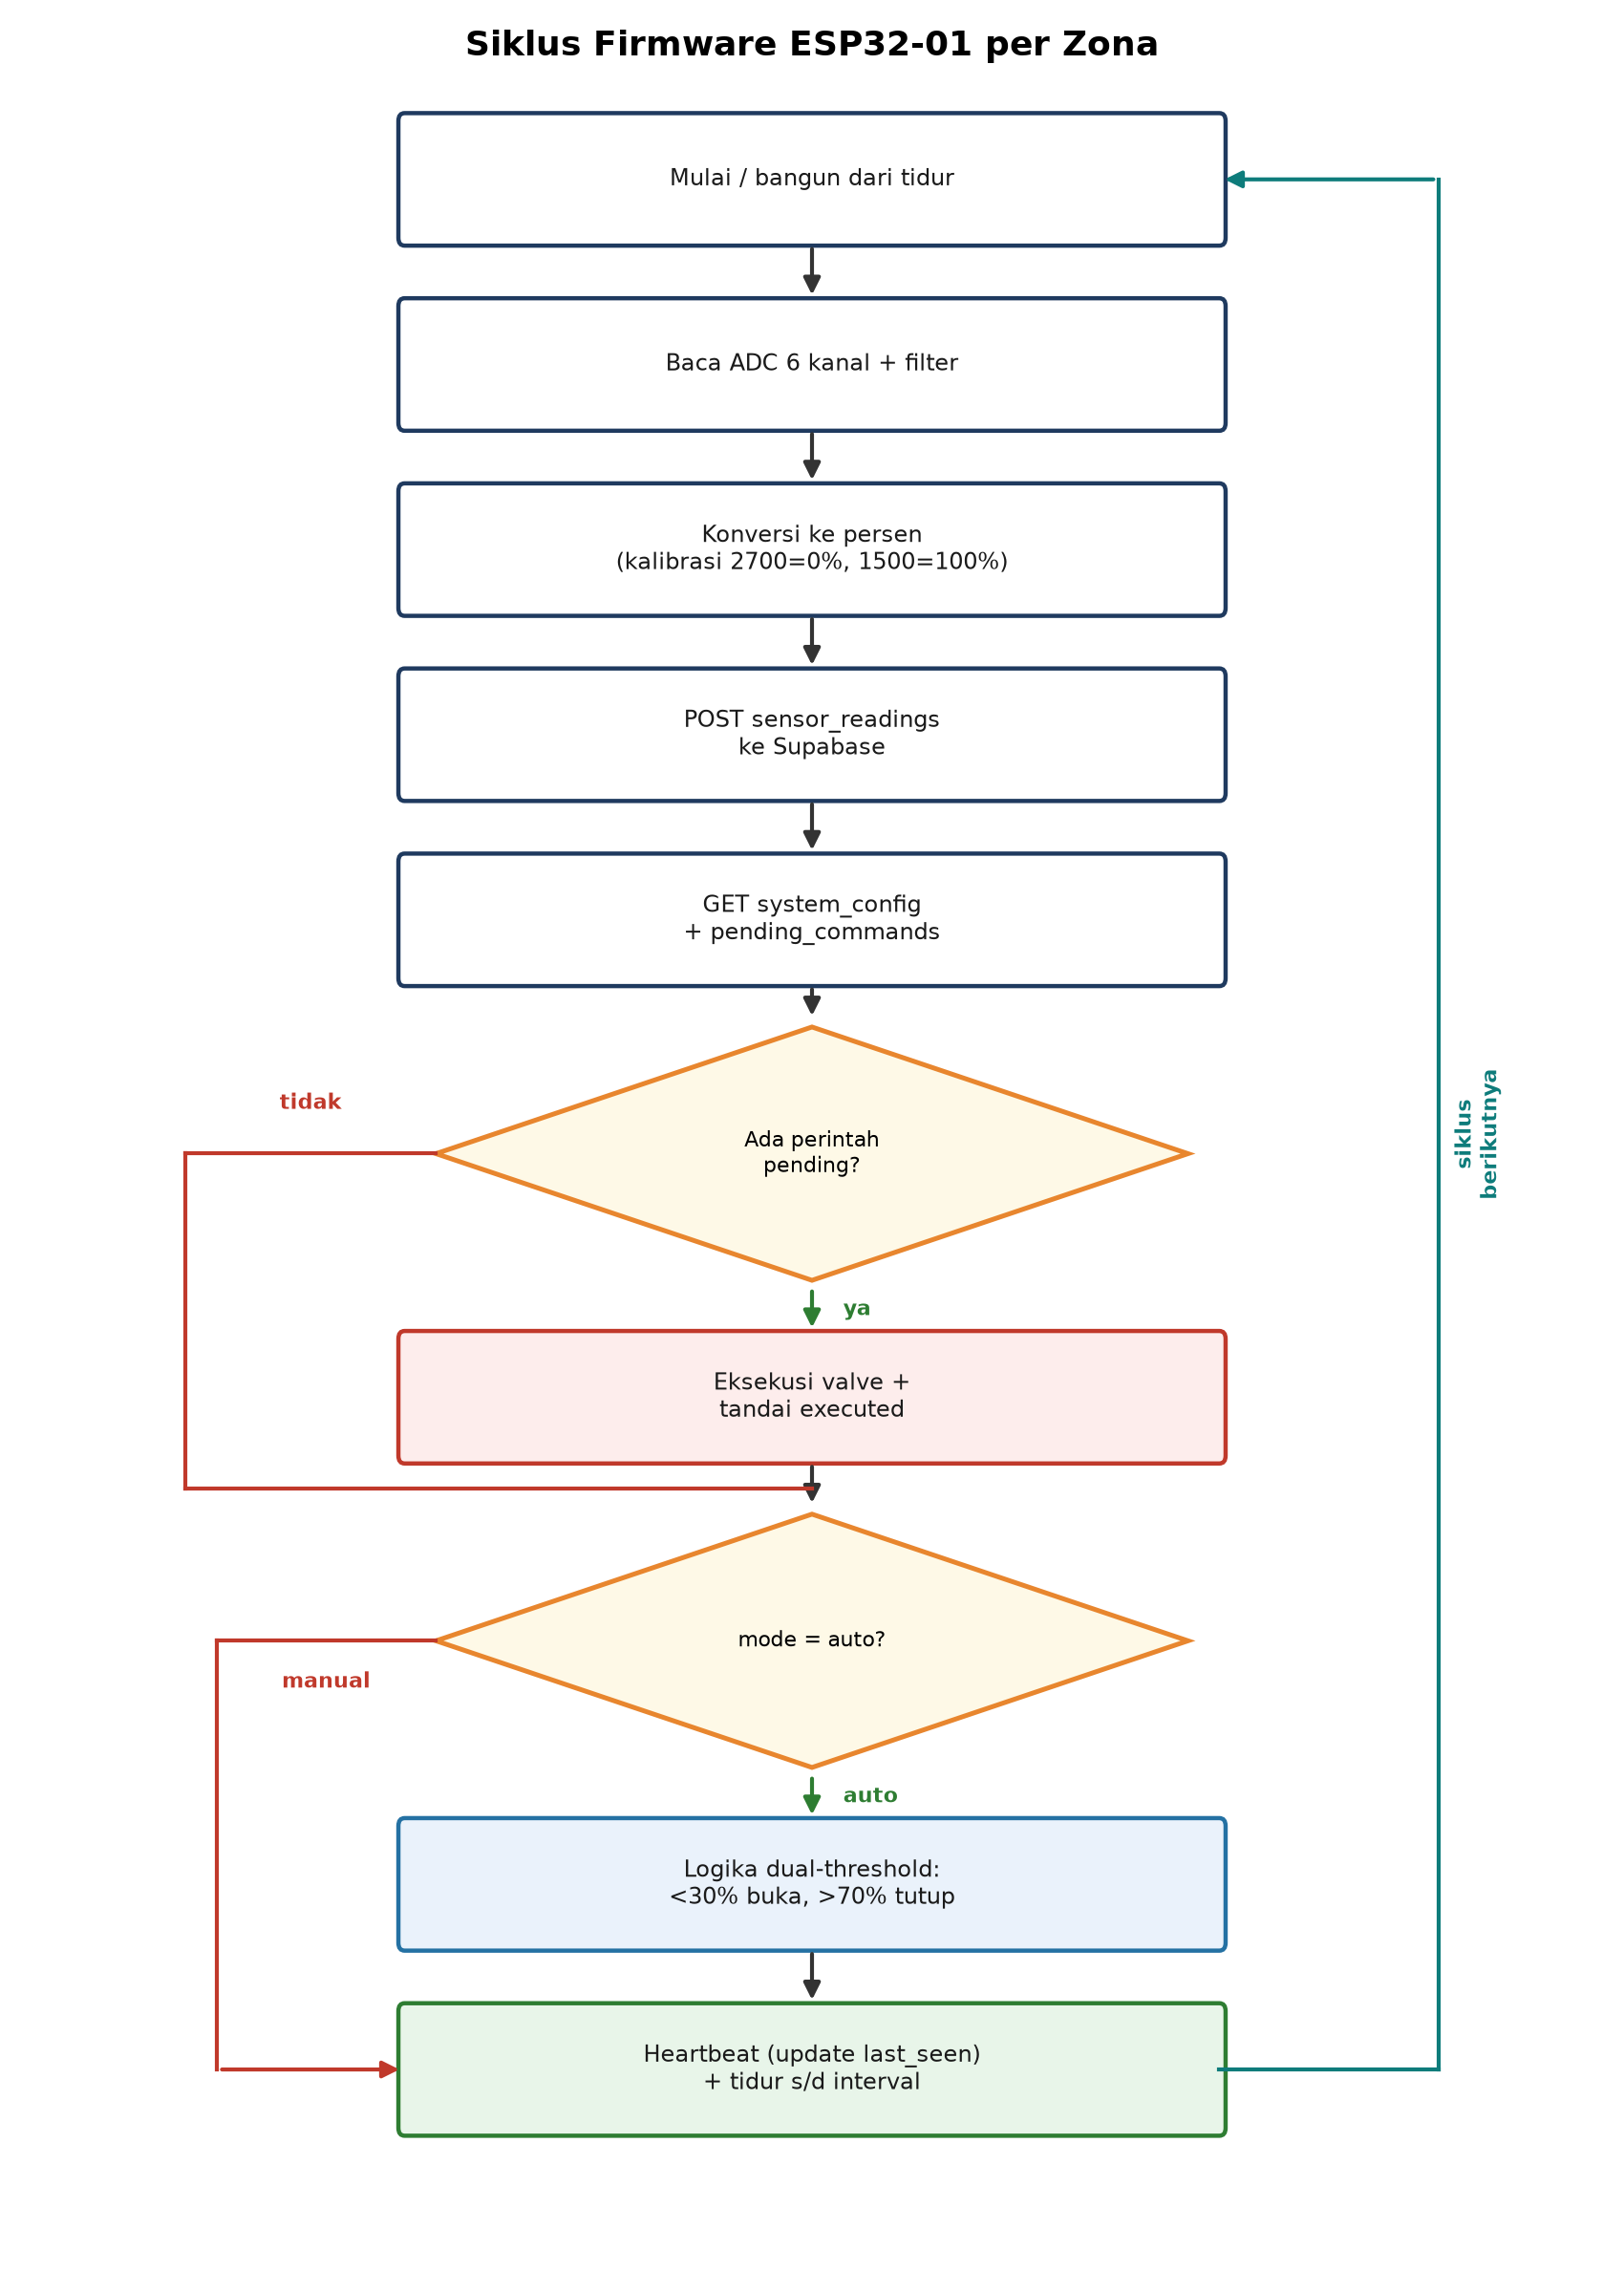
\includegraphics[height=0.78\textheight,keepaspectratio]{figures/fig2_firmware.png}
\caption{Siklus firmware ESP32-01 per zona: bangun, baca 6 kanal ADC, konversi, POST bacaan, GET konfigurasi dan antrean perintah, eksekusi perintah manual bila ada, logika dual-threshold bila mode auto, heartbeat, lalu tidur. Jalur merah adalah bypass (tidak ada perintah / mode manual).}
\label{fig:firmware}
\end{figure}

\section{Backend (Skema Data)}
Empat tabel sebagaimana Bab 2. Aturan penting: status perintah hanya satu dari \textit{pending/executed/expired/cancelled}; ADC valid 100--4000; konfigurasi default per zona adalah mode=auto, threshold\_dry=30, threshold\_wet=70, valve\_duration=30 detik, read\_interval=1800 detik. Fungsi RPC \textit{heartbeat(esp32\_id)} memperbarui \textit{last\_seen} seluruh petak node tersebut.

\begin{figure}[h]
\centering
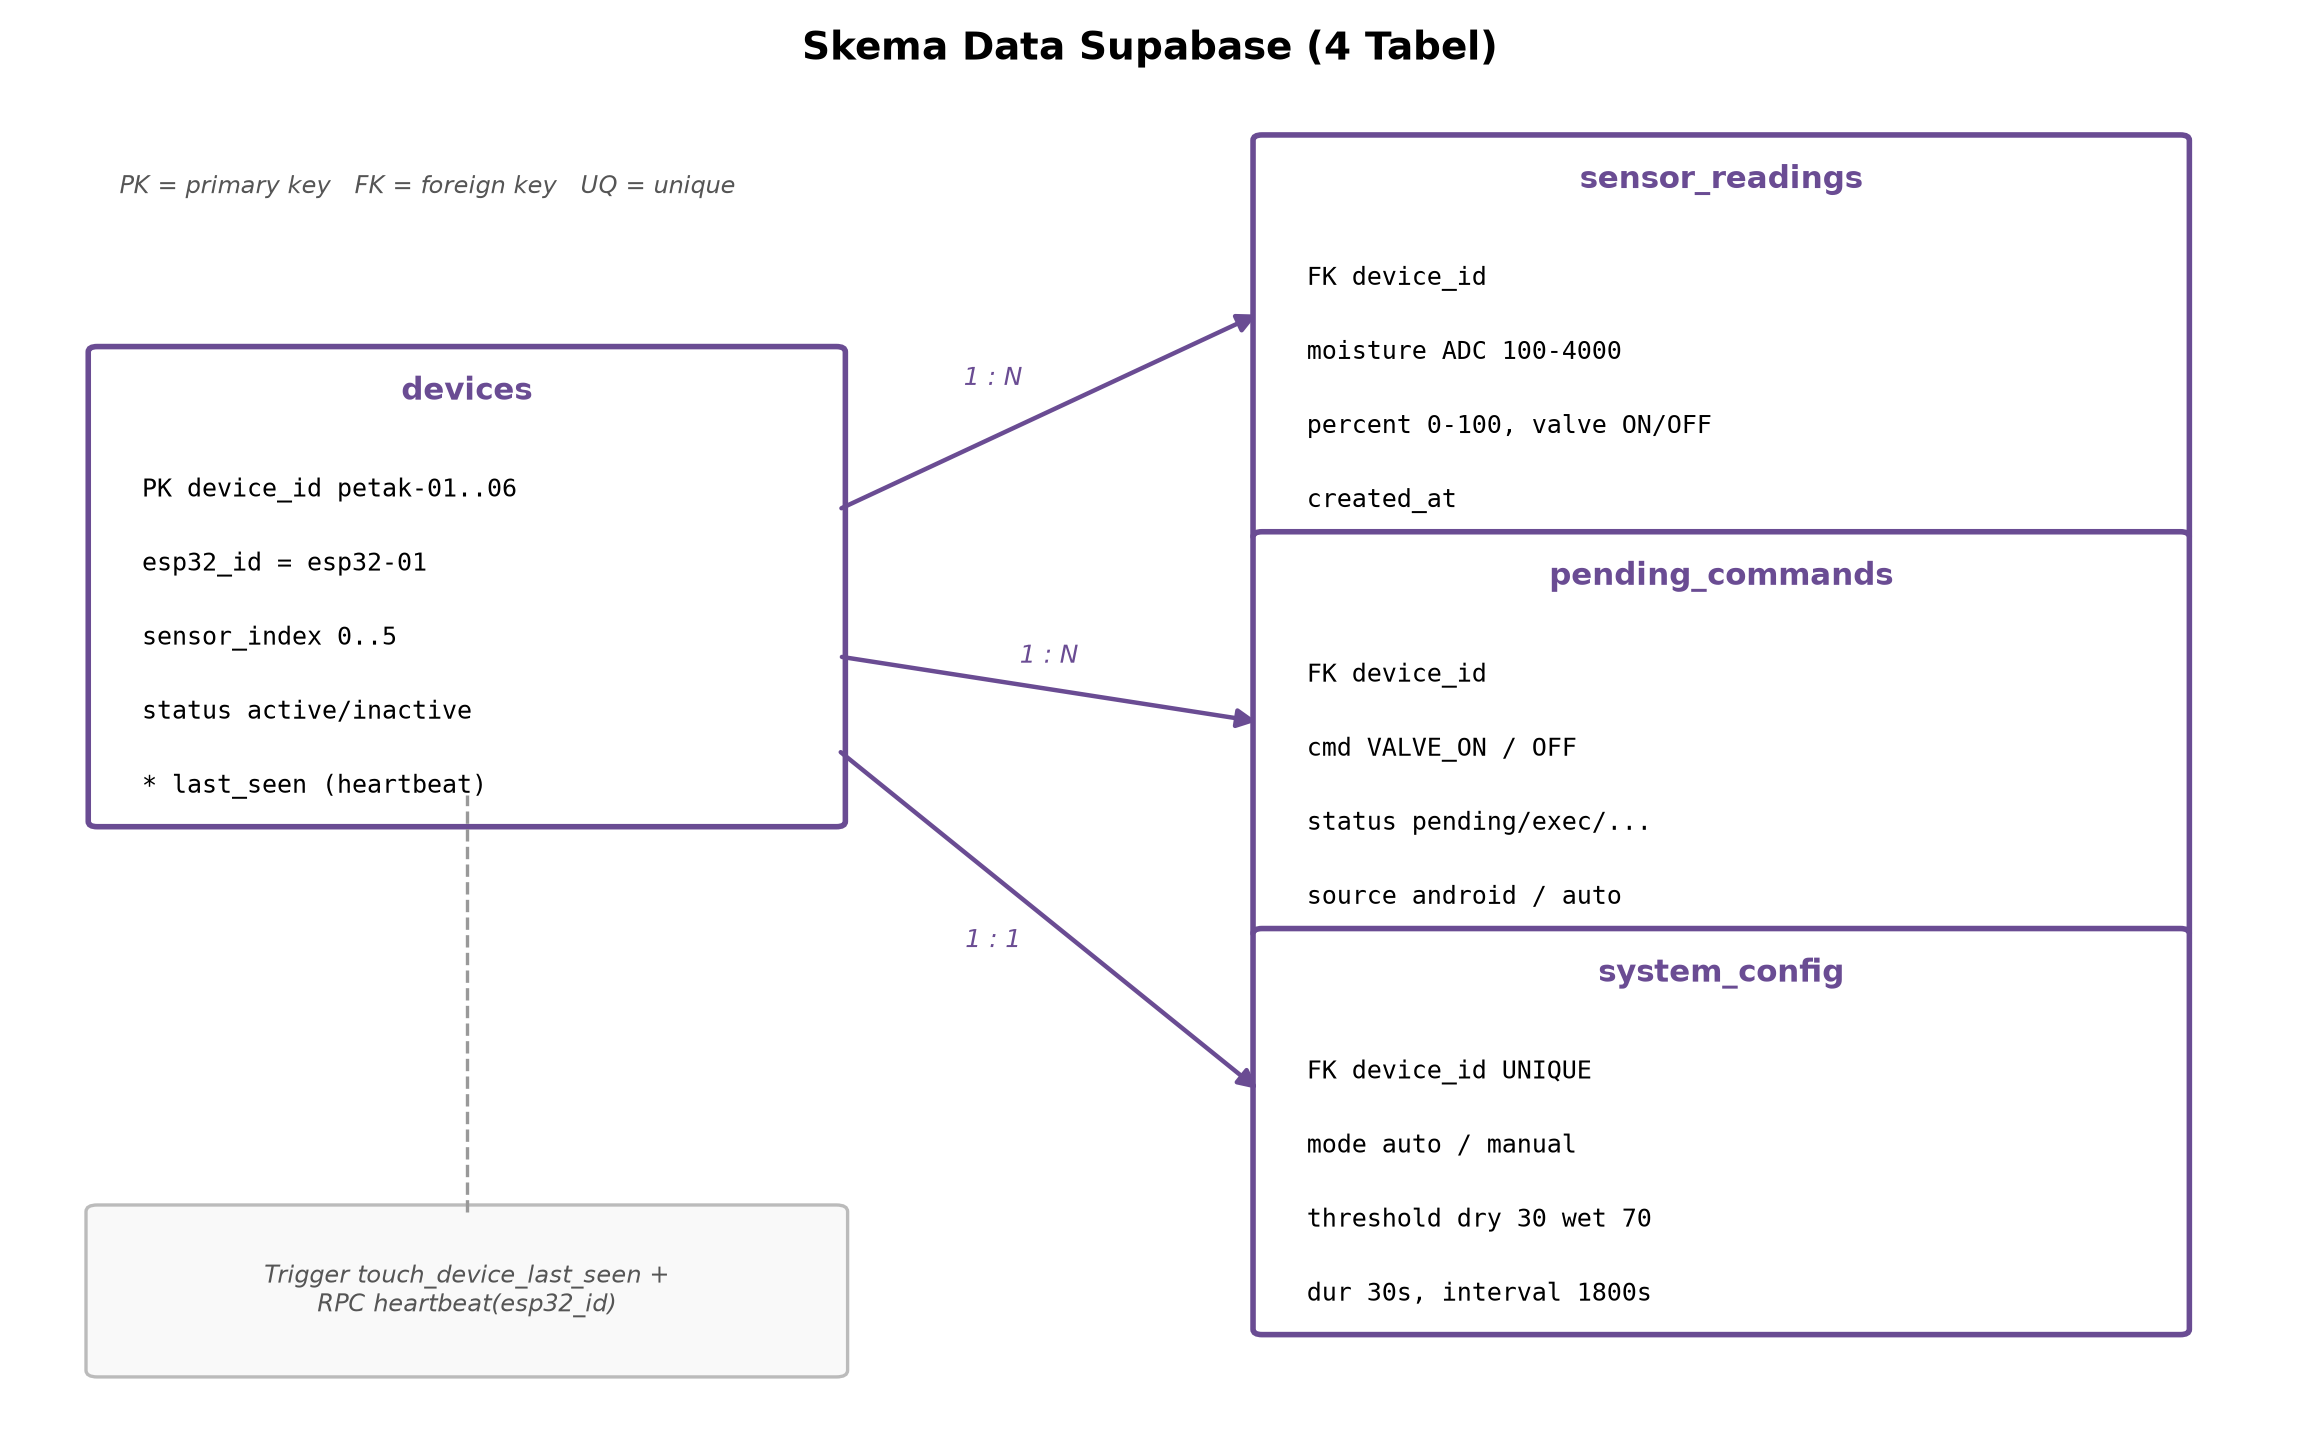
\includegraphics[width=\textwidth]{figures/fig3_database.png}
\caption{Skema data Supabase: \textit{devices} sebagai induk 6 petak, berelasi 1:N ke \textit{sensor\_readings} dan \textit{pending\_commands}, serta 1:1 ke \textit{system\_config}. Kolom \textit{last\_seen} diperbarui via trigger dan RPC heartbeat.}
\label{fig:database}
\end{figure}

\section{Aplikasi Android}
Fitur v0.2.0: dasbor real-time per petak, kontrol BUKA/TUTUP, mode auto/manual, pengaturan threshold, grafik historis jujur (sumbu-x berbasis waktu; SENSOR ERROR tidak di-plot), cuaca 7 hari + rekomendasi (tunda siram jika peluang hujan $\geq$60\%; waspada panas $\geq$33$^{\circ}$C dan kering), jurnal kegiatan + pustaka 10 artikel (lokal), rekapan semua sensor (statistik + batang), dan offline mode (snapshot cache + banner + tombol valve dinonaktifkan saat luring).

\section{Kalibrasi Sensor}
Dua titik di tanah lahan: kering udara ($\approx$ADC 2700) dan jenuh air ($\approx$ADC 1500), diverifikasi per sensor karena variasi unit; rentang valid 100--4000 ditegakkan di firmware dan database.

\section{Rancangan Pengujian}
\begin{table}[h]
\centering
\caption{Rancangan pengujian dan kriteria lolos.}
\begin{tabularx}{\textwidth}{llX}
\toprule
Kode & Aspek & Metode dan kriteria \\
\midrule
P1 & Fungsional valve & 10 perintah BUKA/TUTUP per zona via aplikasi; lolos jika 100\% dieksekusi dan tercatat executed. \\
P2 & Akurasi threshold & Tanah dikeringkan/dibasahi melewati 30\% dan 70\%; lolos jika aksi valve sesuai logika dan tanpa chattering ($\geq$5 siklus). \\
P3 & Latensi perintah & Ukur HP $\rightarrow$ Supabase $\rightarrow$ ESP32 $\rightarrow$ valve; target median $<$15 detik pada 4G. \\
P4 & Akurasi heartbeat & Matikan/hidupkan ESP32 terjadwal; lolos jika status aplikasi benar $\geq$95\% sampel. \\
P5 & Efisiensi air & Bandingkan volume air 14 hari vs penyiraman manual terjadwal pada petak kontrol; hipotesis hemat $\geq$40\%. \\
P6 & Keberterimaan & SUS ke $\geq$10 petani; target skor $\geq$70. \\
\bottomrule
\end{tabularx}
\end{table}

\section{Jadwal Penelitian (8 minggu)}
\begin{table}[h]
\centering
\begin{tabularx}{\textwidth}{Xcccccccc}
\toprule
Kegiatan & 1 & 2 & 3 & 4 & 5 & 6 & 7 & 8 \\
\midrule
Kalibrasi sensor + rakit 6 zona & $\times$ & $\times$ & & & & & & \\
Integrasi Supabase + firmware & & $\times$ & $\times$ & & & & & \\
Uji P1--P4 (lab + lahan) & & & & $\times$ & $\times$ & & & \\
Uji P5 (14 hari) + SUS & & & & & $\times$ & $\times$ & & \\
Analisis + tulis makalah & & & & & & & $\times$ & $\times$ \\
Submit semnas & & & & & & & & $\times$ \\
\bottomrule
\end{tabularx}
\end{table}

% ================= BAB 4 =================
\chapter{Hasil yang Diharapkan dan Luaran}

Target: (1) prototipe 6 zona beroperasi off-grid di Desa Merayan; (2) bukti kuantitatif P1--P6; (3) makalah seminar nasional 6--8 halaman + presentasi; (4) APK Android dan repositori terbuka; (5) dataset pembacaan sensor 14 hari. Indikator keberhasilan minimal: P1 100\%, P2 tanpa chattering, P4 $\geq$95\%, SUS $\geq$70, dan penghematan air terukur positif signifikan.

% ================= PUSTAKA =================
\begin{thebibliography}{99}
\addcontentsline{toc}{chapter}{Daftar Pustaka}

\bibitem{abdelmoneim2025} A. Abdelmoneim dkk., ``Calibration of low-cost capacitive soil moisture sensors for irrigation management applications,'' \textit{Sensors}, vol. 25, no. 2, p. 343, Jan. 2025. DOI: 10.3390/s25020343.

\bibitem{saputri2025} F. R. Saputri, R. Linelson, M. Salehuddin, D. M. Nor, dan M. I. Ahmad, ``Design and development of an irrigation monitoring and control system based on blynk internet of things and thingspeak,'' \textit{PLOS ONE}, vol. 20, no. 4, p. e0321250, Apr. 2025. DOI: 10.1371/journal.pone.0321250.

\bibitem{fahrunnisa2026} Z. Fahrunnisa, A. M. N. Imron, I. N. Agiska, W. Muldayani, G. A. Rahardi, dan C. P. R. Ramadhani, ``IoT-based innovative irrigation system for chili using Telegram bot and web dashboard,'' \textit{Journal of Applied Electrical Engineering}, vol. 10, no. 1, 2026. DOI: 10.30871/jaee.v10i1.12251.

\bibitem{espressif-datasheet} Espressif Systems, ``ESP32 series datasheet.'' Tersedia: \url{https://documentation.espressif.com/esp32_datasheet_en.pdf}. Diakses Okt. 2026.

\bibitem{supabase-docs} Supabase, ``Supabase documentation.'' Tersedia: \url{https://supabase.com/docs}. Diakses Okt. 2026.

\bibitem{openmeteo-docs} Open-Meteo, ``Weather forecast API documentation.'' Tersedia: \url{https://open-meteo.com/en/docs}. Diakses Okt. 2026. Gratis tanpa API key, data terbuka CC BY 4.0.

\bibitem{fao-drip} FAO, ``Climate-smart agriculture technology catalogue: drip irrigation,'' Repositori OpenKnowledge FAO. Tersedia: \url{https://openknowledge.fao.org/bitstreams/3b089d91-bf20-4e51-8d59-789b6abf0ec0/download}. Diakses Okt. 2026.

\end{thebibliography}

\end{document}
